\documentclass[10pt]{article}
\usepackage[margin=0.75in]{geometry}
\usepackage{graphicx}
\usepackage{amsmath}
\usepackage{hyperref}
\usepackage{enumitem}
\usepackage{tikz}
\usepackage{xcolor}
\usetikzlibrary{shapes,arrows,positioning}

% Statistics removed - no longer auto-generated

\title{\textbf{Solstice: LLM-Orchestrated System for Medical Document Fact-Checking}}
\author{An AI-Native Approach to Evidence Extraction and Verification}
\date{}

\begin{document}
\maketitle

\section{Introduction}

Solstice is a multi-step system that automatically fact-checks medical claims against scientific literature and clinical documents. It combines layout detection, multimodal language models, and an orchestrated chain of LLM calls to extract and verify evidence from PDFs that contain text, tables, and figures.

The system is designed to handle real-world medical documentation at scale, processing complex clinical documents containing text, tables, and figures.

\section{System Architecture}

\subsection{Document Ingestion Pipeline}

The ingestion pipeline transforms unstructured PDFs into queryable structured documents through multiple stages:

\begin{enumerate}[leftmargin=*,topsep=0pt,itemsep=0pt]
\item \textbf{Layout Detection}: Uses Detectron2 with PubLayNet-trained models (Mask R-CNN + ResNet-50-FPN). The pipeline relies on pre-trained weights rather than custom training because PubLayNet provides extensive annotated data.
\item \textbf{Box Consolidation}: Merges overlapping layout detections and resolves conflicts. Medical PDFs often contain complex overlapping elements that require special handling.
\item \textbf{Text Extraction}: Uses PyMuPDF for vector text extraction within bounding boxes.
\item \textbf{Figure/Table Extraction}: Saves visual elements as PNG at 400 DPI. Images are stored separately for later multimodal analysis rather than embedded as base64.
\item \textbf{Reading Order}: Computes reading order with column detection and vertical positioning; this is necessary for the multi-column layouts common in medical journals.
\end{enumerate}

\subsection{LLM-Based Fact-Checking System}

The fact-checking pipeline processes text evidence through three sequential stages (Extract → Completeness → Verify) followed by parallel image analysis:

\begin{itemize}[leftmargin=*,topsep=0pt]
\item \textbf{Evidence Extraction Step}: Searches document text for claim-relevant quotes using gpt-4.1. Preserves exact quotes and returns structured evidence with relevance explanations.

\item \textbf{Completeness Checker}: Reviews the extracted evidence and searches the document again for any additional quotes that weren't initially found, ensuring comprehensive coverage.

\item \textbf{Evidence Verification Step (V2)}: Validates that all extracted quotes (from both extraction and completeness steps) exist in the source document. Uses semantic matching and filters out tangentially related content, achieving high verification rates.

\item \textbf{Image Evidence Analyzer}: Analyzes figures and tables using vision models to identify supporting visual evidence and provide detailed explanations.
\end{itemize}

After all LLM processing completes, an Evidence Presenter step consolidates all verified text and image evidence into structured JSON reports with coverage assessment.

\subsection{LLM Pipeline Flow}

The fact-checking pipeline orchestrates multiple LLM calls in a specific sequence:

\begin{figure}[ht]
\centering
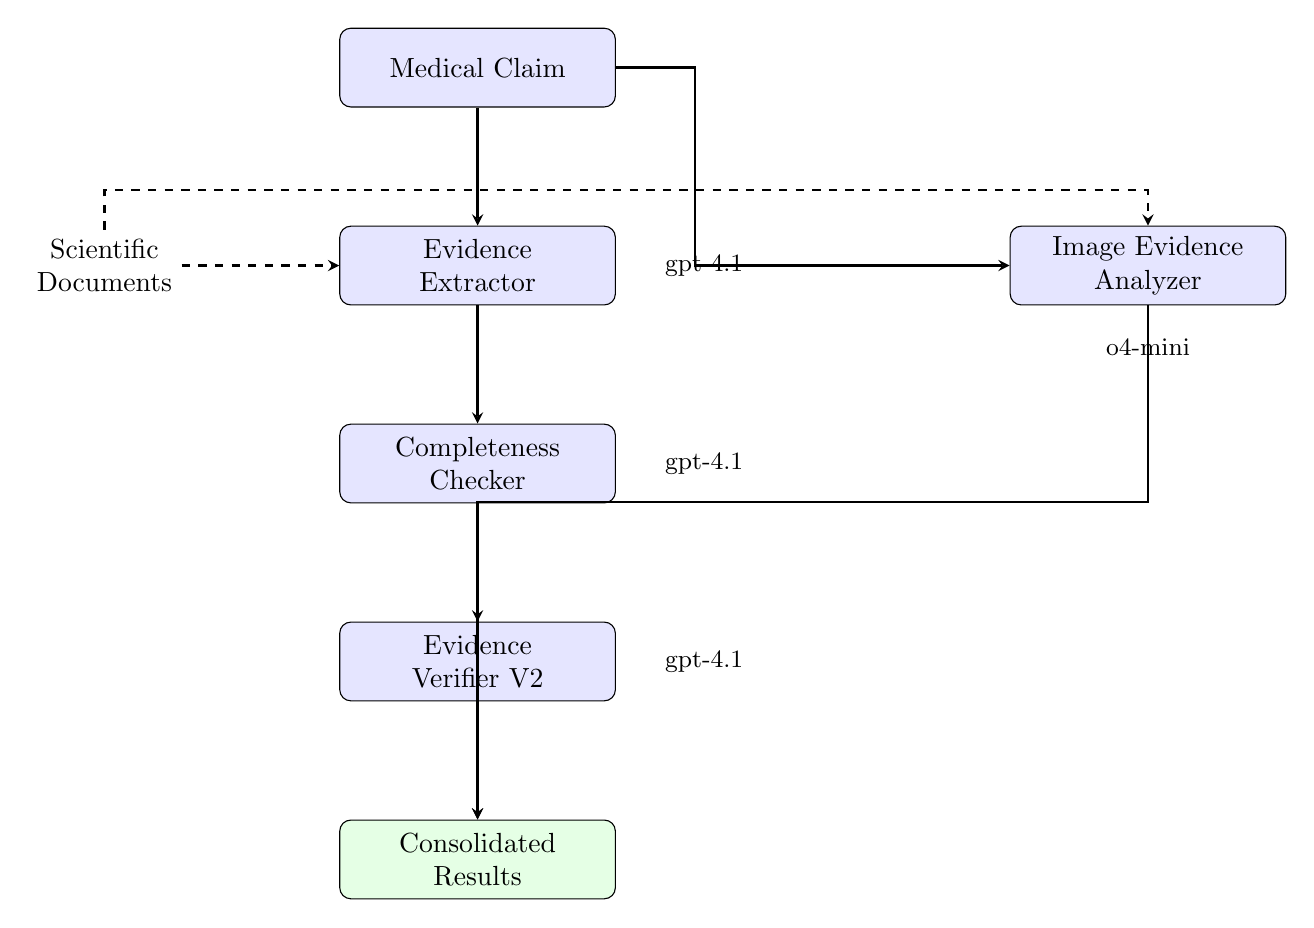
\begin{tikzpicture}[
    node distance=1.5cm,
    box/.style={rectangle, draw, rounded corners, minimum width=3.5cm, minimum height=1cm, align=center, fill=blue!10},
    arrow/.style={thick,->,>=stealth}
]

% Nodes
\node[box] (claim) {Medical Claim};
\node[box, below=of claim] (extract) {Evidence\\Extractor};
\node[box, below=of extract] (complete) {Completeness\\Checker};
\node[box, below=of complete] (verify) {Evidence\\Verifier V2};
\node[box, right=5cm of extract] (image) {Image Evidence\\Analyzer};
\node[box, below=of verify, fill=green!10] (result) {Consolidated\\Results};

% Scientific docs
\node[left=2cm of extract, align=center] (docs) {Scientific\\Documents};

% Arrows
\draw[arrow] (claim) -- (extract);
\draw[arrow] (extract) -- (complete);
\draw[arrow] (complete) -- (verify);
\draw[arrow] (verify) -- (result);
\draw[arrow] (claim.east) -- ++(1,0) |- (image);
\draw[arrow] (image.south) -- ++(0,-2.5) -| (result);
\draw[arrow, dashed] (docs) -- (extract);
\draw[arrow, dashed] (docs.north) -- ++(0,0.5) -| (image);

% Labels
\node[right=0.5cm of extract, font=\small] {gpt-4.1};
\node[right=0.5cm of complete, font=\small] {gpt-4.1};
\node[right=0.5cm of verify, font=\small] {gpt-4.1};
\node[below=0.3cm of image, font=\small] {o4-mini};

\end{tikzpicture}
\caption{LLM Pipeline: Sequential text evidence processing with parallel image analysis}
\end{figure}

\section{Technical Implementation}

\subsection{Core Services Architecture}

Solstice is built on three logical services, with the Gateway service running in Docker for isolation:

\begin{figure}[ht]
\centering
\resizebox{\textwidth}{!}{%
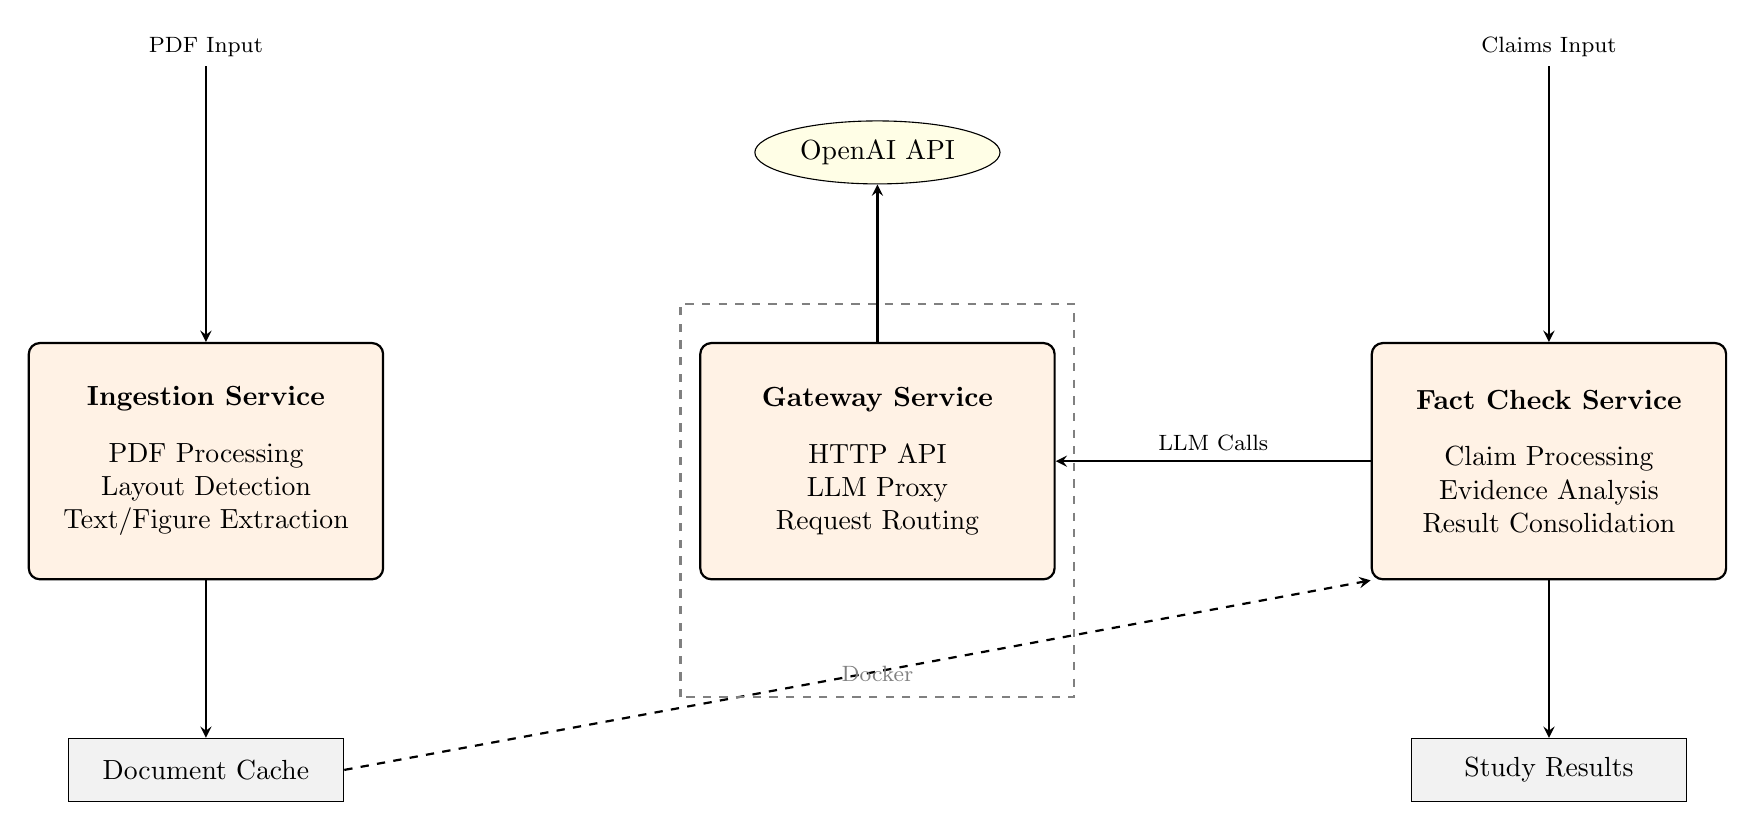
\begin{tikzpicture}[
    node distance=3cm,
    service/.style={rectangle, draw, rounded corners, minimum width=4.5cm, minimum height=3cm, align=center, fill=orange!10, thick},
    component/.style={rectangle, draw, minimum width=3.5cm, minimum height=0.8cm, align=center, fill=gray!10},
    api/.style={ellipse, draw, minimum width=2.5cm, minimum height=0.8cm, align=center, fill=yellow!10},
    arrow/.style={thick,->,>=stealth},
    label/.style={font=\footnotesize}
]

% Gateway Service
\node[service] (gateway) {
    \textbf{Gateway Service}\\[0.3cm]
    HTTP API\\
    LLM Proxy\\
    Request Routing
};

% Ingestion Service
\node[service, left=4cm of gateway] (ingestion) {
    \textbf{Ingestion Service}\\[0.3cm]
    PDF Processing\\
    Layout Detection\\
    Text/Figure Extraction
};

% Fact Check Service
\node[service, right=4cm of gateway] (factcheck) {
    \textbf{Fact Check Service}\\[0.3cm]
    Claim Processing\\
    Evidence Analysis\\
    Result Consolidation
};

% External APIs
\node[api, above=2cm of gateway] (openai) {OpenAI API};

% Data stores
\node[component, below=2cm of ingestion] (cache) {Document Cache};
\node[component, below=2cm of factcheck] (results) {Study Results};

% User entry points
\node[above=3.5cm of ingestion, label] (pdfin) {PDF Input};
\node[above=3.5cm of factcheck, label] (claims) {Claims Input};

% Arrows
\draw[arrow] (pdfin) -- (ingestion);
\draw[arrow] (claims) -- (factcheck);
\draw[arrow] (ingestion) -- (cache);
\draw[arrow] (factcheck) -- (results);
\draw[arrow] (factcheck.west) -- node[label, above] {LLM Calls} (gateway.east);
\draw[arrow] (gateway) -- (openai);
\draw[arrow, dashed] (cache.east) -- (factcheck.south west);

% Docker container box (only for Gateway)
\draw[thick, dashed, gray] (-2.5,-3) rectangle (2.5,2);

\node at (0,-2.7) [label, gray] {Docker};

\end{tikzpicture}
}
\caption{Core Services Architecture: Gateway runs in Docker as the central LLM interface}
\end{figure}

\subsection{Orchestration Layer}

The system uses asynchronous Python with strategic architectural decisions:

\begin{itemize}[leftmargin=*,topsep=0pt,itemsep=0pt]
\item \textbf{Hierarchical Orchestration}: Two-level design with StudyOrchestrator → ClaimOrchestrator → processing steps. Enables both study-level and claim-level parallelism control.
\item \textbf{Step Isolation}: Each processing step runs independently with explicit input/output contracts via Pydantic models. Enables testing and development in isolation.
\end{itemize}

\subsection{Where to Find the Data Artifacts}

Solstice writes intermediate and final results to disk in human-readable form. This allows users to inspect the system, debug individual stages, or create visualisations without rerunning the full pipeline.

\paragraph{1. Fact-Checking Study Results}
After you run a fact-checking study (\texttt{python -m src.cli run-study}), the main results file containing all claims with their supporting text, tables, and figures is located at:

\begin{verbatim}
data/studies/consolidated_results.json
\end{verbatim}

This single JSON file contains all the verified evidence for each claim. Here's the structure with a stubbed example:

\begin{verbatim}
{
  "study_name": "unknown",
  "timestamp": "2025-07-30T23:47:44.122369",
  "claims": [
    {
      "claim": "Flublok ensures identical antigenic match with 
               WHO- and FDA-selected flu strains.",
      "evidence": [
        {
          "type": "text",
          "quote": "The primary amino acid sequence of the rHA 
                   produced using baculovirus...is identical 
                   to the HA from the wild type virus...",
          "explanation": "The quote directly supports the claim...",
          "document": "Arunachalam_et_al.__2021_"
        },
        {
          "type": "image",
          "filename": "figure_p2_det_1_000.png",
          "reasoning": "The table provides data showing Flublok 
                       contains 45 µg HA per strain...",
          "document": "CDC_Influenza_vaccines"
        }
      ]
    },
    {
      "claim": "Flublok contains 3x the hemagglutinin (HA) antigen 
               content of standard-dose flu vaccines...",
      "evidence": [
        // Additional text and image evidence entries
      ]
    }
    // Additional claims...
  ]
}
\end{verbatim}

Each claim contains an array of evidence entries that can be either:
\begin{itemize}[leftmargin=*,topsep=0pt,itemsep=0pt]
\item \textbf{Text evidence}: Exact quotes from documents with explanations of how they support or refute the claim
\item \textbf{Image evidence}: References to figures/tables with reasoning about their relevance
\end{itemize}

The evidence entries always include the source document name, making it easy to trace back to the original PDFs in the scientific or marketing cache.

\paragraph{2. Marketing Material Cache}
Marketing PDFs like FlublokOnePage are processed with special attention to layout preservation. To see the marketing page layout, look at:

\begin{verbatim}
data/marketing_cache/FlublokOnePage/visualizations/page_001_layout.png
\end{verbatim}

This visualization shows the detected layout elements (text blocks, figures, headers) overlaid on the original page, helping verify proper extraction of complex marketing layouts.

The full directory structure for marketing materials:

\begin{verbatim}
data/marketing_cache/FlublokOnePage/
|-- extracted/
|   |-- content.json          # Extracted text and layout structure
|   |-- document.html         # HTML version of the document
|   |-- document.md           # Markdown version
|   |-- document.txt          # Plain text version
|   `-- figures/
|       |-- figure_p1_04314352.png
|       |-- figure_p1_6de74a29.png
|       `-- figure_p1_d9d91bd1.png
|-- pages/
|   `-- page-000.png          # Full page image  
`-- visualizations/
    `-- page_001_layout.png   # ** MARKETING LAYOUT VISUALIZATION **
\end{verbatim}

\paragraph{3. Scientific Document Cache}
Scientific papers undergo the same extraction process but may include additional agent processing for fact-checking. For example, Treanor\_et\_al.\_\_2011\_ contains:

\begin{verbatim}
data/scientific_cache/Treanor_et_al.__2011_/
|-- extracted/
|   |-- content.json          # Extracted text and layout structure
|   |-- document.html         # HTML version
|   |-- document.md           # Markdown version
|   |-- document.txt          # Plain text version
|   `-- figures/              # Extracted figures and tables
|       |-- figure_p1_det_0_005.png
|       |-- figure_p3_det_2_000.png
|       |-- table_p3_det_2_009.png
|       `-- table_p4_det_3_003.png
|-- pages/                    # Individual page images
|   |-- page-000.png
|   |-- page-001.png
|   `-- ...
|-- visualizations/           # Layout detection overlays
|   |-- all_pages_summary.png
|   |-- page_001_layout.png
|   `-- ...
|-- raw_layouts/              # Intermediate layout data
|   `-- raw_layout_boxes.json
`-- agents/                   # Fact-checking results (if processed)
    `-- claims/
        `-- claim_000/
            |-- evidence_extractor/
            |-- completeness_checker/
            `-- evidence_verifier_v2/
\end{verbatim}

The key difference is that scientific documents may have an \texttt{agents/} directory containing fact-checking results for individual claims.

\paragraph{4. Quick Directory Cheatsheet}
For newcomers, these are useful places to explore:
\begin{itemize}[leftmargin=*]
  \item \texttt{src/cli/} – entry-point scripts that orchestrate the pipelines.
  \item \texttt{src/injestion/shared/processing/} – layout detection, reading-order logic, text extractors.
  \item \texttt{src/fact\_check/agents/} – implementation of the four specialised LLM processing steps plus formatting.
  \item \texttt{data/scientific\_cache/} – processed scientific PDFs (inspect \texttt{content.json}).
  \item \texttt{data/marketing\_cache/} – processed marketing PDFs.
  \item \texttt{data/studies/} – end-to-end fact-checking results ready for consumption.
\end{itemize}

\section{Implementation Notes}

\subsection{Model Integration and Multimodal Processing}

The system uses different models for text and image analysis, reflecting a key architectural decision to process these modalities separately:

\subsubsection{Text Processing with gpt-4.1}
All text-based evidence extraction and verification uses gpt-4.1, chosen specifically for its needle-in-haystack capabilities:
\begin{itemize}[leftmargin=*,topsep=0pt,itemsep=0pt]
\item \textbf{Evidence extraction}: Searches through hundreds of pages to find exact quotes matching claims
\item \textbf{High-precision retrieval}: Locates specific sentences in dense medical literature with minimal false positives
\item \textbf{Completeness checking}: Re-scans documents to catch any quotes missed in the first pass
\item \textbf{Exact quote verification}: Confirms extracted text exists verbatim in source documents
\end{itemize}

\subsubsection{Image Analysis with o4-mini}
Visual evidence (figures, tables, charts) is processed using o4-mini, a reasoning model chosen for its ability to interpret complex visual information:
\begin{itemize}[leftmargin=*,topsep=0pt,itemsep=0pt]
\item \textbf{Visual reasoning}: Interprets data trends, statistical significance, and relationships shown in charts
\item \textbf{Table comprehension}: Understands structured data and can identify relevant rows/columns supporting claims
\item \textbf{Diagram analysis}: Reasons about flowcharts, mechanisms, and visual explanations of processes
\item \textbf{Contextual interpretation}: Understands what visual evidence actually demonstrates in context
\end{itemize}

\subsubsection{Why Separate Text and Image Processing?}
Processing text and images separately leverages the distinct strengths of different model types:

\begin{enumerate}[leftmargin=*,topsep=0pt,itemsep=0pt]
\item \textbf{Model specialization}: gpt-4.1 excels at needle-in-haystack tasks—finding specific quotes in massive documents—while reasoning models like o4-mini are better at interpreting visual information and drawing conclusions
\item \textbf{Task optimization}: Text evidence extraction is fundamentally a search and retrieval problem where precision matters most. Image analysis requires reasoning about relationships, trends, and visual patterns
\item \textbf{Prompt engineering}: Extraction tasks benefit from deterministic responses while visual reasoning tasks need more flexible interpretation
\item \textbf{Performance characteristics}: gpt-4.1 can process enormous text contexts efficiently for quote extraction, while reasoning models handle the cognitive load of understanding charts, diagrams, and data visualizations
\end{enumerate}

\subsubsection{Technical Implementation}
\begin{itemize}[leftmargin=*,topsep=0pt,itemsep=0pt]
\item All LLM calls route through an HTTP gateway service for centralized request handling
\item Images are stored as files (not base64) for easier inspection and debugging
\item Parallel image processing is limited to prevent overwhelming the API
\item Both pipelines use structured JSON schemas for predictable output formats
\end{itemize}

\subsection{Three-Stage Text Evidence Pipeline}
Extraction, verification, and completeness are run as distinct LLM-driven steps:
\begin{itemize}[leftmargin=*,topsep=0pt,itemsep=0pt]
\item \textbf{Stage 1}: Extract all potentially relevant quotes (high recall)
\item \textbf{Stage 2}: Find additional quotes not caught in initial extraction (expand coverage)
\item \textbf{Stage 3}: Verify all quotes exist and support claim (high precision)
\end{itemize}
This separation allows the stages to be optimised and tested independently.

\subsection{Filesystem-Centric Architecture}
The pipeline stores intermediate data on the filesystem rather than in a database:
\begin{itemize}[leftmargin=*,topsep=0pt,itemsep=0pt]
\item Human-readable JSON can be inspected without extra tools
\item Hierarchical directories (document/claim/step) reflect the processing flow
\item No additional infrastructure is required
\item Files can be version-controlled in Git
\end{itemize}


\section{Conclusion}

Solstice combines layout understanding, multimodal analysis, and orchestrated LLM calls to perform medical fact-checking. Tests on multiple documents and claims indicate that the architecture can process real-world medical documentation at moderate scale.

\end{document}
